\documentclass[12pt,letterpaper]{article}
\usepackage{fullpage}
\usepackage[top=2cm, bottom=4.5cm, left=2.5cm, right=2.5cm]{geometry}
\usepackage{amsmath,amsthm,amsfonts,amssymb,amscd}
\usepackage{lastpage}
\usepackage{enumerate}
\usepackage{fancyhdr}
\usepackage{mathrsfs}
\usepackage{xcolor}
\usepackage{graphicx}
\usepackage{listings}
\usepackage{hyperref}
\usepackage[utf8]{inputenc}
\usepackage{tikz}
\hypersetup{%
  colorlinks=true,
  linkcolor=blue,
  linkbordercolor={0 0 1}
}
 
\renewcommand\lstlistingname{Algorithm}
\renewcommand\lstlistlistingname{Algorithms}
\def\lstlistingautorefname{Alg.}

\lstdefinestyle{Python}{
    language        = Python,
    frame           = lines, 
    basicstyle      = \footnotesize,
    keywordstyle    = \color{blue},
    stringstyle     = \color{green},
    commentstyle    = \color{red}\ttfamily
}

\setlength{\parindent}{0.0in}
\setlength{\parskip}{0.05in}

% Edit these as appropriate
\newcommand\course{Intelligence artificielle}
\newcommand\hwnumber{1}                  % <-- homework number
\newcommand\NetIDa{}           % <-- NetID of person #1
\newcommand\NetIDb{}           % <-- NetID of person #2 (Comment this line out for problem sets)

\pagestyle{fancyplain}
\headheight 35pt
\lhead{\small ENSA-Fès}
% \lhead{\NetIDa\\\NetIDb}                 % <-- Comment this line out for problem sets (make sure you are person #1)
\chead{\textbf{\Large Homework \hwnumber}}
\rhead{\course \\ \today}
\lfoot{}
\cfoot{}
\rfoot{\small\thepage}
\headsep 1.5em

\begin{document}

\section*{Description de l'environnement}%
\label{sec:description_de_l_environnement}
Donner une \textbf{formulation} complète \footnote{assez précise pour être
  implémentée} du problème pour chacun des situations
suivantes:

\begin{itemize}
  \item Soit \textbf{six} boites en verre alignées, chacune munie d'une serrure.
    Les cinq premierès contiennent chacune une \textbf{clé} qui permet d'ouvrir
    la boite \emph{suivante}; la dérnière boite contient une \textbf{banane}.
    Vous avez la clé de la première boite et vous voulez obtenir la banane.

  \item Vous commencer par la séquence \textbf{ABABAECCEC}, ou plus
    généralement n'importe quelle séquence composée de $A$, de $B$, de $C$
    et de $E$. Vous pouvez transformer cette séquence en appliquant les
    égalités suivantes: $AC=E$, $AB=BC$, $BB=E$ et $Ex=x$ pour n'importe
    quel $x$. Par exemple $ABBC$ peut être transformée en $AEC$, puis $AC$,
    puis $E$. Votre objectif est d'atteindre la séquence $\mathbf{E}$.
  \item Soit un sol constitué d'une grille $n \times n$ de carrés, chaque
    carré étant initialement \textbf{non peint} (sans fond). Au début, vous
    êtes sur  un carré non peint; vous pouvez peindre le carré sur votre
    emplacement ou se déplacer à un carré non peint \emph{adjacent}. Votre
    objectif est de peindre tout le sol.
\end{itemize}


\section*{Arbre de recherche }%
\label{sec:probleme_1}
 Compter le nombre de noeuds dans l'arbre d'exploration \textbf{complet} pour
 le graphe présenté dans. 

\begin{figure}[htpb]
  \centering
  \tikzstyle{simpleNode}=[circle,draw,thick,minimum width=0.8cm] 

\begin{tikzpicture}[xscale=4,->=stealth]

  \node[simpleNode] (s) at (0,0) {$S$};
  \node[simpleNode] (b) at (1,0) {$B$};
  \node[simpleNode] (a) at (2,0) {$A$};
  \node[simpleNode] (g) at (3,0.5) {$G$};
  \node[simpleNode] (c) at (0.5,1) {$C$};

  \path[->,draw,thick](s)--(b);
  \path[->,draw,thick](b)--(a);
  \path[->,draw,thick](a)--(g);
  \path[->,draw,thick](s)--(c);
  \path[->,draw,thick](c)--(b);
  \path[->,draw,thick](s) to[bend right=60](a);

\end{tikzpicture}

  \caption{Graphe du problème}
  \label{fig:q1_graph}
\end{figure}


\section*{Depth-First Search}%
\label{sec:depth_first_search}
\begin{itemize}
  \item 
Exécuter la recherche en \emph{profondeur} (DFS) dans le graphe de la
Figure~\ref{fig:q1_graph}. On considère les noeuds selon leurs ordre
\emph{alphabétique} (i.e. Le plan $S\rightarrow X \rightarrow A$ sera considéré avant le plan
$S\rightarrow X\rightarrow B$). Il est fortement recommandé d'exécuter la recherche dans un
Brouillon.

\item Donner le chemin choisi par (DFS).
\end{itemize}

\section*{Breadth-First Search}%
\label{sec:}

\begin{itemize}
  \item 
Exécuter la recherche en \emph{largeur} (BFS) dans le graphe de la
Figure~\ref{fig:q1_graph}. On considère les noeuds selon leurs ordre
\emph{alphabétique} (i.e. Le plan $S\rightarrow X \rightarrow A$ sera considéré avant le plan
$S\rightarrow X\rightarrow B$). Il est fortement recommandé d'exécuter la recherche dans un
Brouillon.

\item Donner le chemin choisi par (BPS).
\end{itemize}


\section*{Uniform Cost Search}%
\label{sec:uniform_cost_search}


\begin{itemize}
  \item 
Exécuter la recherche uniforme en coût (UCS) dans le graphe de la
  
Figure~\ref{fig:q4_graph}. On considère les noeuds selon leurs ordre
\emph{alphabétique} (i.e. Le plan $S\rightarrow X \rightarrow A$ sera considéré avant le plan
$S\rightarrow X\rightarrow B$). \end{itemize}

\begin{figure}[htpb]
  \centering
  
\tikzstyle{simpleNode}=[circle,draw,very thick,minimum width=0.8cm] 

\begin{tikzpicture}[xscale=4,->=stealth]

  \node[simpleNode] (s) at (0,0) {$S$};
  \node[simpleNode] (b) at (1,-1) {$B$};
  \node[simpleNode] (a) at (1,1) {$A$};
  \node[simpleNode] (c) at (2,1) {$C$};
  \node[simpleNode] (g) at (3,0) {$G$};
  \node[simpleNode] (d) at (2,-1) {$D$};
  \path[->,draw,thick] (s)--(a)node[midway,above]{$2$};
  \path[->,draw,thick] (s)--(b)node[midway,below]{$1$};
  \path[->,draw,thick] (a)--(c)node[midway,above]{$3$};
  \path[->,draw,thick] (b)--(d)node[midway,above]{$5$};
  \path[->,draw,thick] (a)--(b)node[midway,left]{$1$};
  \path[->,draw,thick] (a)--(d)node[midway,above]{$1$};
  \path[->,draw,thick] (c)--(g)node[midway,above]{$7$};
  \path[->,draw,thick] (d)--(g)node[midway,above]{$4$};
  \path[->,draw,thick] plot[smooth] coordinates {(b.south) (2,-1.8)(g.south)};
  \node at (2,-2){$10$};
    
\end{tikzpicture}

  \caption{Graphe Pondéré}
  \label{fig:q4_graph}
\end{figure}


\section*{Recherche Optimale $A^*$}%
\label{sec:recherche_optimale_a_}

Dans cette question on ajoute une \emph{heuristique} au graphe pondéré de la figure~\ref{fig:q4_graph}.

\begin{figure}[htpb]
  \centering
  

\tikzstyle{simpleNode}=[circle,draw,very thick,minimum width=0.8cm, text
width=0.8cm,align =center]

\begin{tikzpicture}[xscale=4,->=stealth]

  \node[simpleNode] (s) at (0,0) {$S$};
  \node[simpleNode] (b) at (1,-1) {$B$ \scriptsize  $h=3$};
  \node[simpleNode] (a) at (1,1) { $B$ \scriptsize $h=3$};
  \node[simpleNode] (c) at (2,1) {$C$ \scriptsize $h=1$};
  \node[simpleNode] (g) at (3,0) {$G$};
  \node[simpleNode] (d) at (2,-1) {$D$ \scriptsize $h=2$};
  \path[->,draw,thick] (s)--(a)node[midway,above]{$2$};
  \path[->,draw,thick] (s)--(b)node[midway,below]{$1$};
  \path[->,draw,thick] (a)--(c)node[midway,above]{$3$};
  \path[->,draw,thick] (b)--(d)node[midway,above]{$5$};
  \path[->,draw,thick] (a)--(b)node[midway,left]{$1$};
  \path[->,draw,thick] (a)--(d)node[midway,above]{$1$};
  \path[->,draw,thick] (c)--(g)node[midway,above]{$7$};
  \path[->,draw,thick] (d)--(g)node[midway,above]{$4$};
  \path[->,draw,thick] plot[smooth] coordinates {(b.south) (2,-2)(g.south)};
  \node at (2,-2.1){$10$};
    
\end{tikzpicture}

  \caption{Graphe pondéré avec heuristique}
  \label{fig:q4_graph}
\end{figure}
\begin{itemize}
    \item Exécuter la recherche optimale $A^*$ et donner l'ordre des
      développement des neodus.
    \item Donner le chemin choisi par $A^*$.
\end{itemize}


\section*{Missionnaires et cannibales}%
\label{sec:missionnaires_et_cannibales}
Le problèmes des \emph{missionnaires et
cannibales} est habituellement énoncé
comme suit: Trois Missionnaires et trois cannibales se trouvent au bord d'une
rivière. avec un bateau qui peut contenir une ou deux personnes. Trouvez une
manière de faire passer tout le monde de l'autre coté sans que jamais un groupe
de missionnaires soit quelque part en présence d'un nombre \textbf{supérieur} de
cannibales. Ce problème est cèlèbre en
IA\footnote{https://en.wikipedia.org/wiki/Missionaries\_and\_cannibals\_problem}
parce que cétait le premier article abordant la formulation de problème d'un
point de vue analytique.

\begin{itemize}
  \item Formulez le problème avec précision, en faisant les distinctions
    nécessaire pour être sûr d'obtenir une solution valide.

  \item Tracez un diagramme de l'ensembre de l'espace des états.
  \item Implémentez et résolvez ce problème en appelant un algorithme
    d'exploration approprié.
\end{itemize}

\section*{Problème Labyrinthe}%
\label{sec:section_name}
Dans les questions suivantes, vous contrôlez un \emph{insecte} dans un
Labyrinthe rectangulaire de dimensions $\mathbf{M,N}$, présenté dans la figure~\ref{fig:maze}. Dans chaque
itération, l'insecte peut se déplacer dans un carré vide ou elle peut choisir de
grader sa position actuelle. Tous les déplacements seront pénalisé par un coût
$c=1$.

\begin{figure}[htpb]
  \centering
  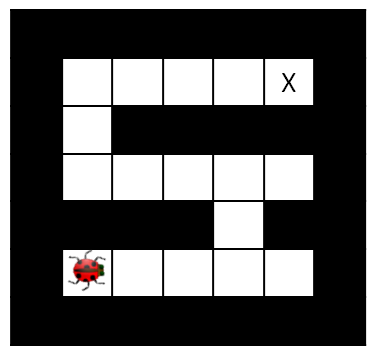
\includegraphics[width=8cm,height=6cm]{./hw1_maze1.png}
  \caption{Labyrinthe}
  \label{fig:maze}
\end{figure}
\subsection*{Un seul insecte}%
\label{sub:un_seul_insecte}

Vous contrôlez un seul insecte, Figure~\ref{fig:maze}, et vous voulez atteindre
le point désigné par $X$ (la ruche). 

\begin{enumerate}
  \item Quel sera la description \textbf{minimale} de votre environnement.
    \begin{itemize}
      \item[$\square$] Un entier $d$ qui représente la distance de Manhattan de
        la ruche.
      \item[$\square$] Un couple $(x,y)$ représentant la position de l'insecte.
      \item[$\square$] Un triplet $(x,y,d)$ représentant la position de
        l'insecte ainsi que la distance à la ruche.
      \item[$\square$] Ce problème ne peut pas être représenté.
    \end{itemize}
  \item Quelle sera la taille de votre environnement en fonction de $N$ et $M$.
  \item Selectionner les \emph{heuristiques} admissible pour ce problème.
    \begin{itemize}
      \item[$\square$] La distance de Manhattan à la ruche.
      \item[$\square$] La distance de Euclidienne à la ruche.
      \item[$\square$] Le nombre de pas pris par l'insecte.

    \end{itemize}
\end{enumerate}

\end{document}
